\documentclass{beamer}
\usetheme{Frankfurt}

\usepackage{graphicx}

\usepackage{url}

\title{The Search for a Universal Turing Machine}
\author{Steven Dee, Justin Gray, Josh Lee, Neil Sandburg}
\date{\today}

\begin{document}

\frame{\titlepage}

\section[Outline]{}
\frame{
	\frametitle{Overview}
	\tableofcontents
}

\section{Team Members and Roles}
\frame{
	\frametitle{Team Members and Roles}
	\begin{itemize}
		\item {\bf Steve Dee:} Database managment, fitness evaluation algorithm
		\item {\bf Justin Gray:} Genetic Algorithm implementation
		\item {\bf Josh Lee:} Turing Machine modeling
		\item {\bf Neil Sandburg:} Web visualization 
	\end{itemize}
}

\section{Overall Objectives}
\frame{
	\frametitle{Overall Objectives}
	Can we use the discovery of Universal Turing Machines as an analogy for the evolution of complex organisms? 
	\begin{columns}
		\begin{column}{.75\textwidth}
			\begin{itemize}
				\item Test the possibility of discovering a set of Unvirsal Turing Machines via a Genetic Algorithm optimization
					\begin{itemize} 
						\item Short optimization with a limited run time
						\item Long optimization with a much longer run time
					\end{itemize}
				\item Create a web application to publish the results of the optimziation
					\begin{itemize}
						\item Real-time link to database being populated by optimization results
						\item Allow user submission of turing machine to test if it exists in the current population
					\end{itemize}
			\end{itemize}
		\end{column}
		\begin{column}{.25\textwidth}
			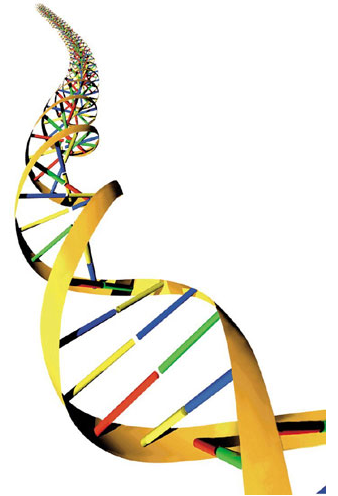
\includegraphics[width=\textwidth]{images/dna.png}
		\end{column}
	\end{columns}
}



\section{Progress Report}
\subsection{Schedule}
\frame{
	\frametitle{Schedule}
	\resizebox{\textwidth}{!}{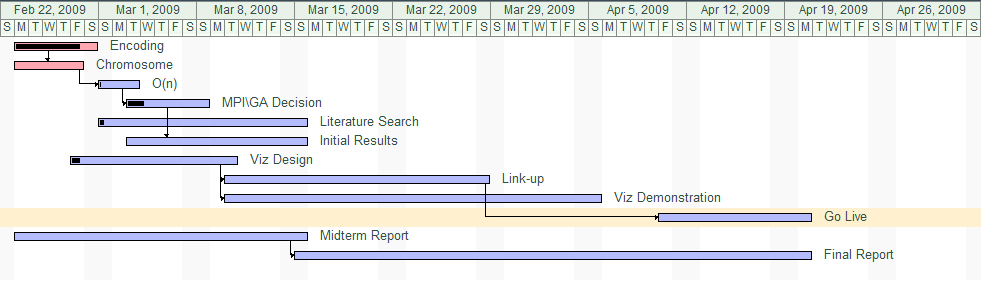
\includegraphics{images/gantt.png}}
	\begin{itemize}
		\item {\bf Encoding}:	Definition of the encoding method for Turing Machines completed
		\item {\bf Chromosome}: Implementation of the chromosome class for the AI4R Genetic Algorithm package completed.
		\item {\bf Initial Results}: Initial Turing Machine Optimization run completed. Data analyzed to ensure the viability of optimization scheme
		\item {\bf Go Live}: Ruby on Rails visualization application goes live with link to genetic algorithm running perpetually.
	\end{itemize}

}

\subsection{Progress}
\frame{
	\frametitle{Progress}
	Genetic Algorithm Optimization:
	\begin{itemize}
		\item Turing Machine implementation
		\item Genetic Encoding: a set of 5 tuples, representing the state transition table of a turing machine
		\item Selection of a Genetic Algorithm: AI4R (\url{http://ai4r.rubyforge.org/})
		\item Chromosomal implemenation begun
			\begin{itemize}
				\item initialization function complete
				\item fitness scoring algorithm established: score based on adaptabilitys
			\end{itemize}
	\end{itemize}
	Web Visualization App:
	\begin{itemize}
		\item Population database created
		\item Conceptual design begun
	\end{itemize}
}

\subsection{Risk Assesment}
\frame{
	\frametitle{Risk Assesment}
	\begin{itemize}
		\item Nothing interesting happens: No interesting TM's result from any of the optimizations. We don't have time to develop a new fitness scoring algorithm and test it.
		\item Something interesting happens, but we don't recognize it: Our literature search turns up UTM's, but none of them show up in optimization. TM's that do turn up appear to be very ``adaptable'', so they might be UTM's. 
		\item Time constraints: may not have enough time to implement the web visualization tool. 
	\end{itemize}
	
}

\end{document}
